\chapter{Model 3D  urządzenia i fotografie stanowiska testowego}

\begin{figure}[H]
    \centering
    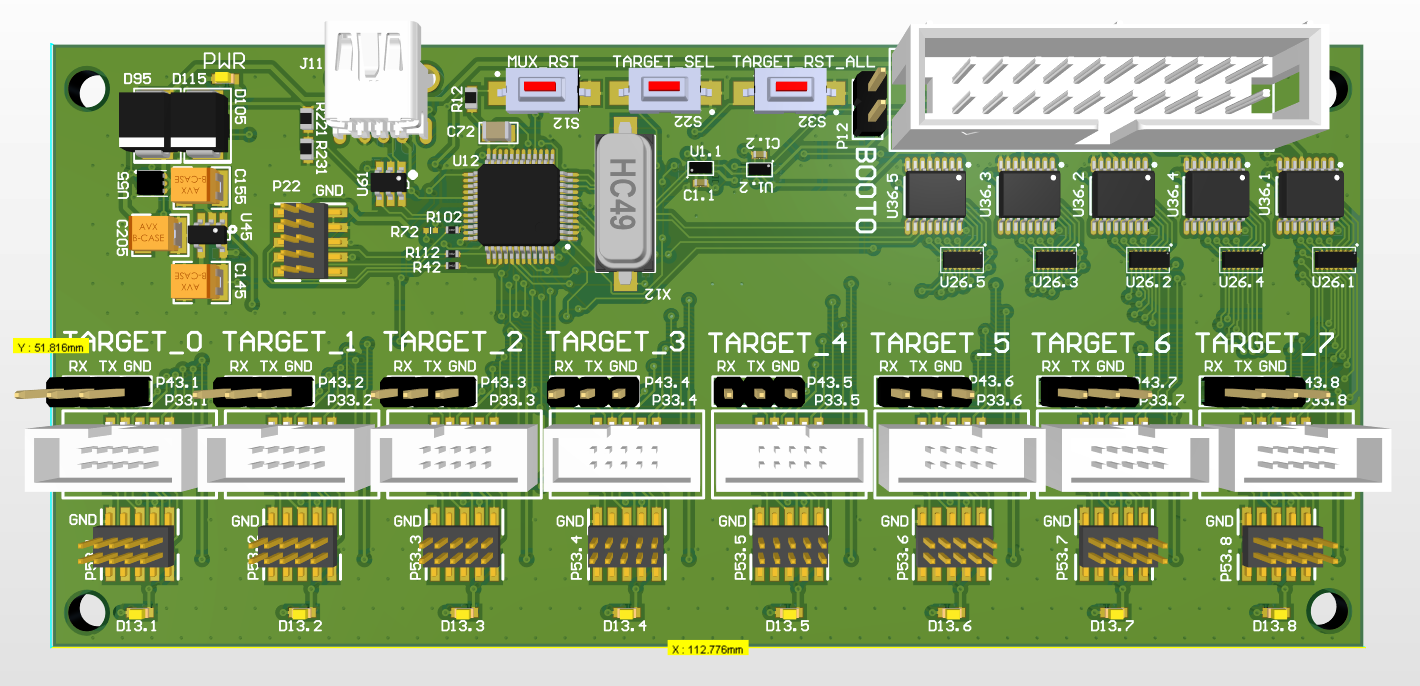
\includegraphics[width=0.75\paperwidth]{images/front_PCB.png}
    \caption{Model 3D płyty PCB widziany od przodu}
    \label{PCB_front}
\end{figure}

\begin{figure}[H]
    \centering
    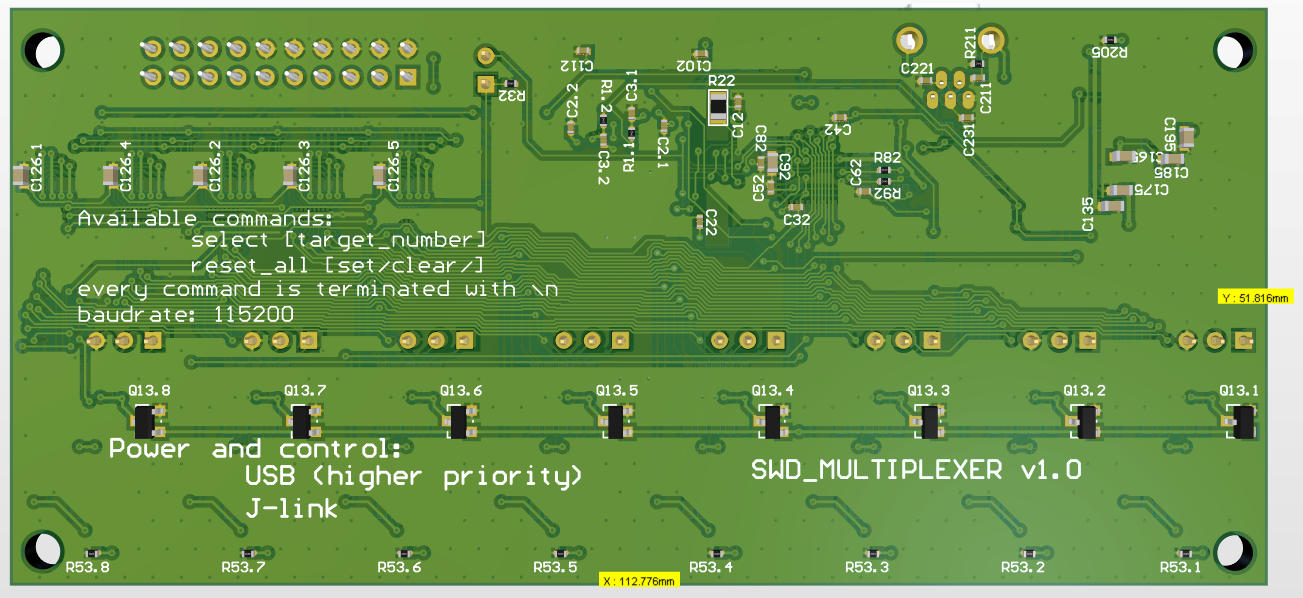
\includegraphics[width=0.75\paperwidth]{images/back_PCB.png}
    \caption{Model 3D płyty PCB widziany od tyłu}
    \label{PCB_back}
\end{figure}

\begin{figure}[H]
    \centering
    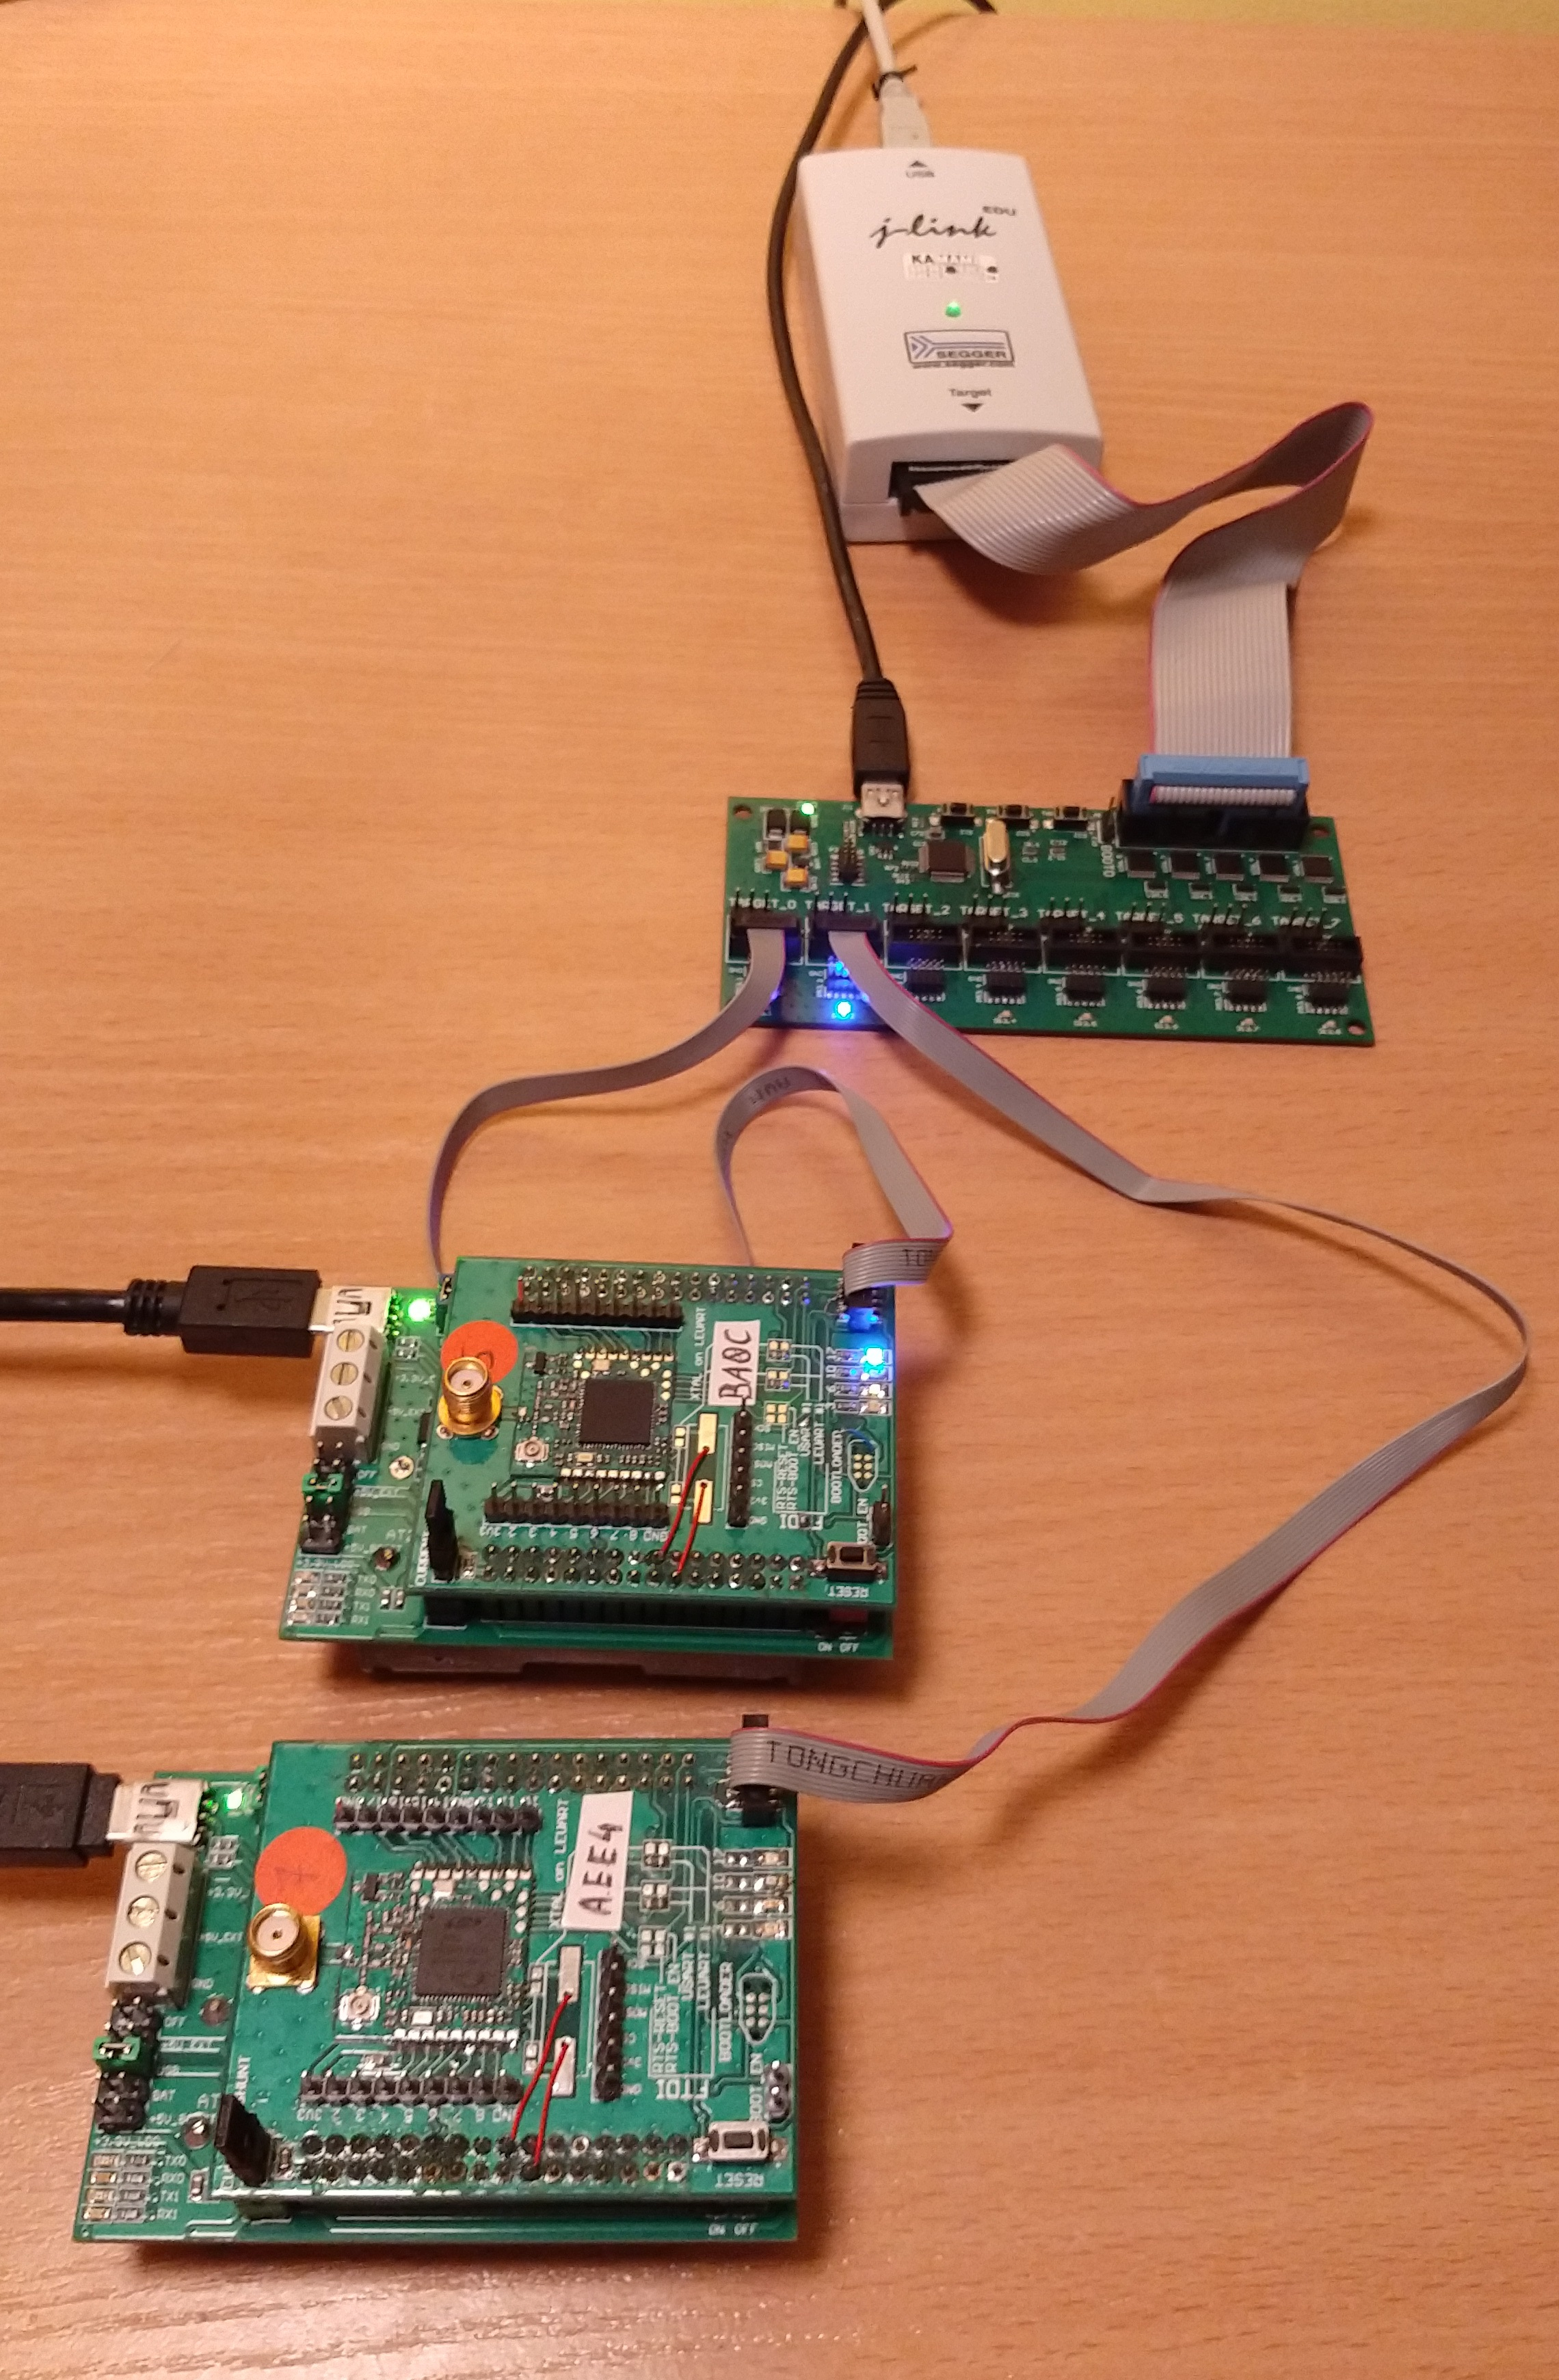
\includegraphics[width=0.75\paperwidth]{images/test_bench.jpg}
    \caption{Zdjęcie stanowiska testowego}
    \label{testbench_photo}
\end{figure}